\documentclass[]{scrartcl}
\usepackage{Preamble}
\usepackage{tikz}
\usepackage{pstricks}

\setcounter{section}{7}
\newcommand{\exercise}{Exercise \thesection}
\newcommand{\duedate}{2021-01-25, 23:59}

\begin{document}
\section*{\exercise}

\subsection{Reading}
\subsection{n-Body Problem --- Partitioning/Communication Design}
\subsubsection{Memory Layout}

\begin{minted}{c++}
  std::random_device rd;  //Will be used to obtain a seed for the random number engine
  std::mt19937 gen(rd()); //Standard mersenne_twister_engine seeded with rd()
  std::uniform_real_distribution<> mass_distrib(1e-10, 1e10);
  std::uniform_real_distribution<> space_distrib(-1e4, 1e4); // start within 25km of eachother

  struct Body {
    union {
      double raw[4];
      struct __attribute__((__packed__)) {
        double m;
        double pos[3];
      };
    };

    Body() {
      m = mass_distrib(gen);
      for (int i=0; i < 3; i++) {
        pos[i] = space_distrib(gen);
      }
    }
  }

  // to send we just use the raw data
  MPI_Send(&b, 8, ...)
\end{minted}

\begin{itemize}
  \item this structure will result in contiguous arrays of bytes which can be sent by their \verb|double raw[4]| representation
  \item velocities will not be sent
  \item \verb|MPI_Gather()| will then collect blocks of mulitple bodies per rank
\end{itemize}

\subsubsection{Partitioning}

\begin{itemize}
  \item the amount of bodies should be a multiple of the available ranks, resulting in equally large messages
  \item each rank will handle a number of bodies
  \item the initial positions and masses are scattered over the ranks
  \item ranks are sequential over nodes (per-slot-mapping) resulting in the least amount of node-to node communication due to circular messaging ($\frac{4}{16}$ of all communication for 16 ranks over 4 nodes)
\end{itemize}

\subsubsection{Communication}
\begin{itemize}
  \item the communication will happen in  a circular fashion
  \item for each arriving packet a copy will be saved inside of a buffer
  \item the now buffered msg can be forwarded to the next rank
  \item while waiting for the arrival of the next msg, the received data can be used to update the Forces on each body the specific rank is responsible for
\end{itemize}

\begin{figure}[H]
  \centering
  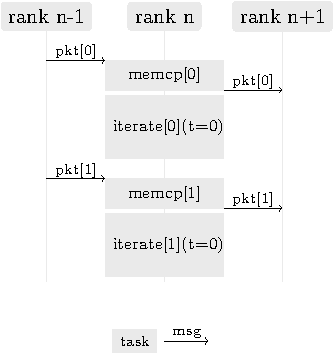
\includegraphics[width=.6\columnwidth]{./img/msg_seq.pdf}
  \caption{Overalp utilization during ring-wise message passing}
  \label{fig:msg_seq}
\end{figure}

\autoref{fig:msg_seq} shows this sequence for a rank n:
\begin{itemize}
  \item here rank n starts out with a running \verb|MPI_Irecv()| and waits for \verb|pkt[0]|
  \item after copying the received data to a buffer, rank n calls \verb|MPI_Isend()| on \verb|pkt[0]| and starts another \verb|MPI_Irecv()|
  \item after iterating over the received data, rank n will wait again for \verb|pkt[1]|
\end{itemize}
\end{document}
